\documentclass[a4paper,12pt,twoside]{article}
\usepackage[T1]{fontenc}
\usepackage[utf8]{inputenc}
\usepackage{lmodern}
\usepackage[american]{babel}
\usepackage{url,csquotes}
\usepackage[hidelinks,hyperfootnotes=false]{hyperref}
\usepackage[titlepage,fancysections,pagenumber]{polytechnique}
\usepackage{float}
\usepackage{amsmath}

\title{Speed Typer}
\author{Diego \textsc{Souza} and Ivan \textsc{Padalko}}
\date{}

\begin{document}
	\maketitle
	
	\tableofcontents
	\newpage
	
	\section{Introduction}
		
		Typing races have become pretty common among multiple computer users, specially programmers. While the most common version are those where the user has to type a given phrase (in a sort of a guided version), this project tries to implement a simpler version: where the user must type the maximum quantity of words in English during a given time.
		
	\section{The Game}
	
		The goal of the game is pretty simple: as the name suggests, the user must type as much words as possible in the given time.
	
		\subsection{The Rules}
	 
			This game has very simple rules:
			
			\begin{itemize}
				\item The user is free to type any word he wants;
				\item The valid words are a very large subset of the English dictionary;
				\item The game uses only ASCII characters and is case-insensitive;
				\item Longer correct words provide more points to the user;
				\item However, wrong words makes the user lose points;
				\item Repetitions do not make the user loses points, but they make the word less valuable;
				\item The user is not allowed to copy paste words.
			\end{itemize}
	
			\subsubsection{The Score}
	
				The score, as described in the rules, is given by the following formula:
				\begin{gather*}
					    \mbox{score}(x)= 
					    \begin{cases}
						    \mbox{max}(2\cdot\mbox{len}(x)-3\cdot\mbox{freq}(x), 0) & \text{if } x \in \mbox{dict}\\
						    -\mbox{len}(x) & \text{otherwise}
					    \end{cases}
				\end{gather*}
				Where len($x$) represents the length of the word, freq($x$) represents how many times the word has been typed in this execution of the game and dict represents the set of valid words.
	
	\section{The Implementation of the Game}
		
		\subsection{The Graphical User Interface (GUI)}
		
			The GUI used in this project was based in the Java SWING. The game has for the moment two possible screens: one for the login of the users (and the creation of new ones) and the other for the game itself.
			
			The first one as shown in figure \ref{fig:login} has two fields: the first one for the username and second one for the password. If the username is one of the registered names in the game, the system will try to make an user authentication with it and its password. Otherwise, the game will consider this to be a new user and register a new user with the given password. Due to implementation reasons, the user will be rejected if its password is the empty string or if its name is too big.
			
			\begin{figure}[H]
				\centering
				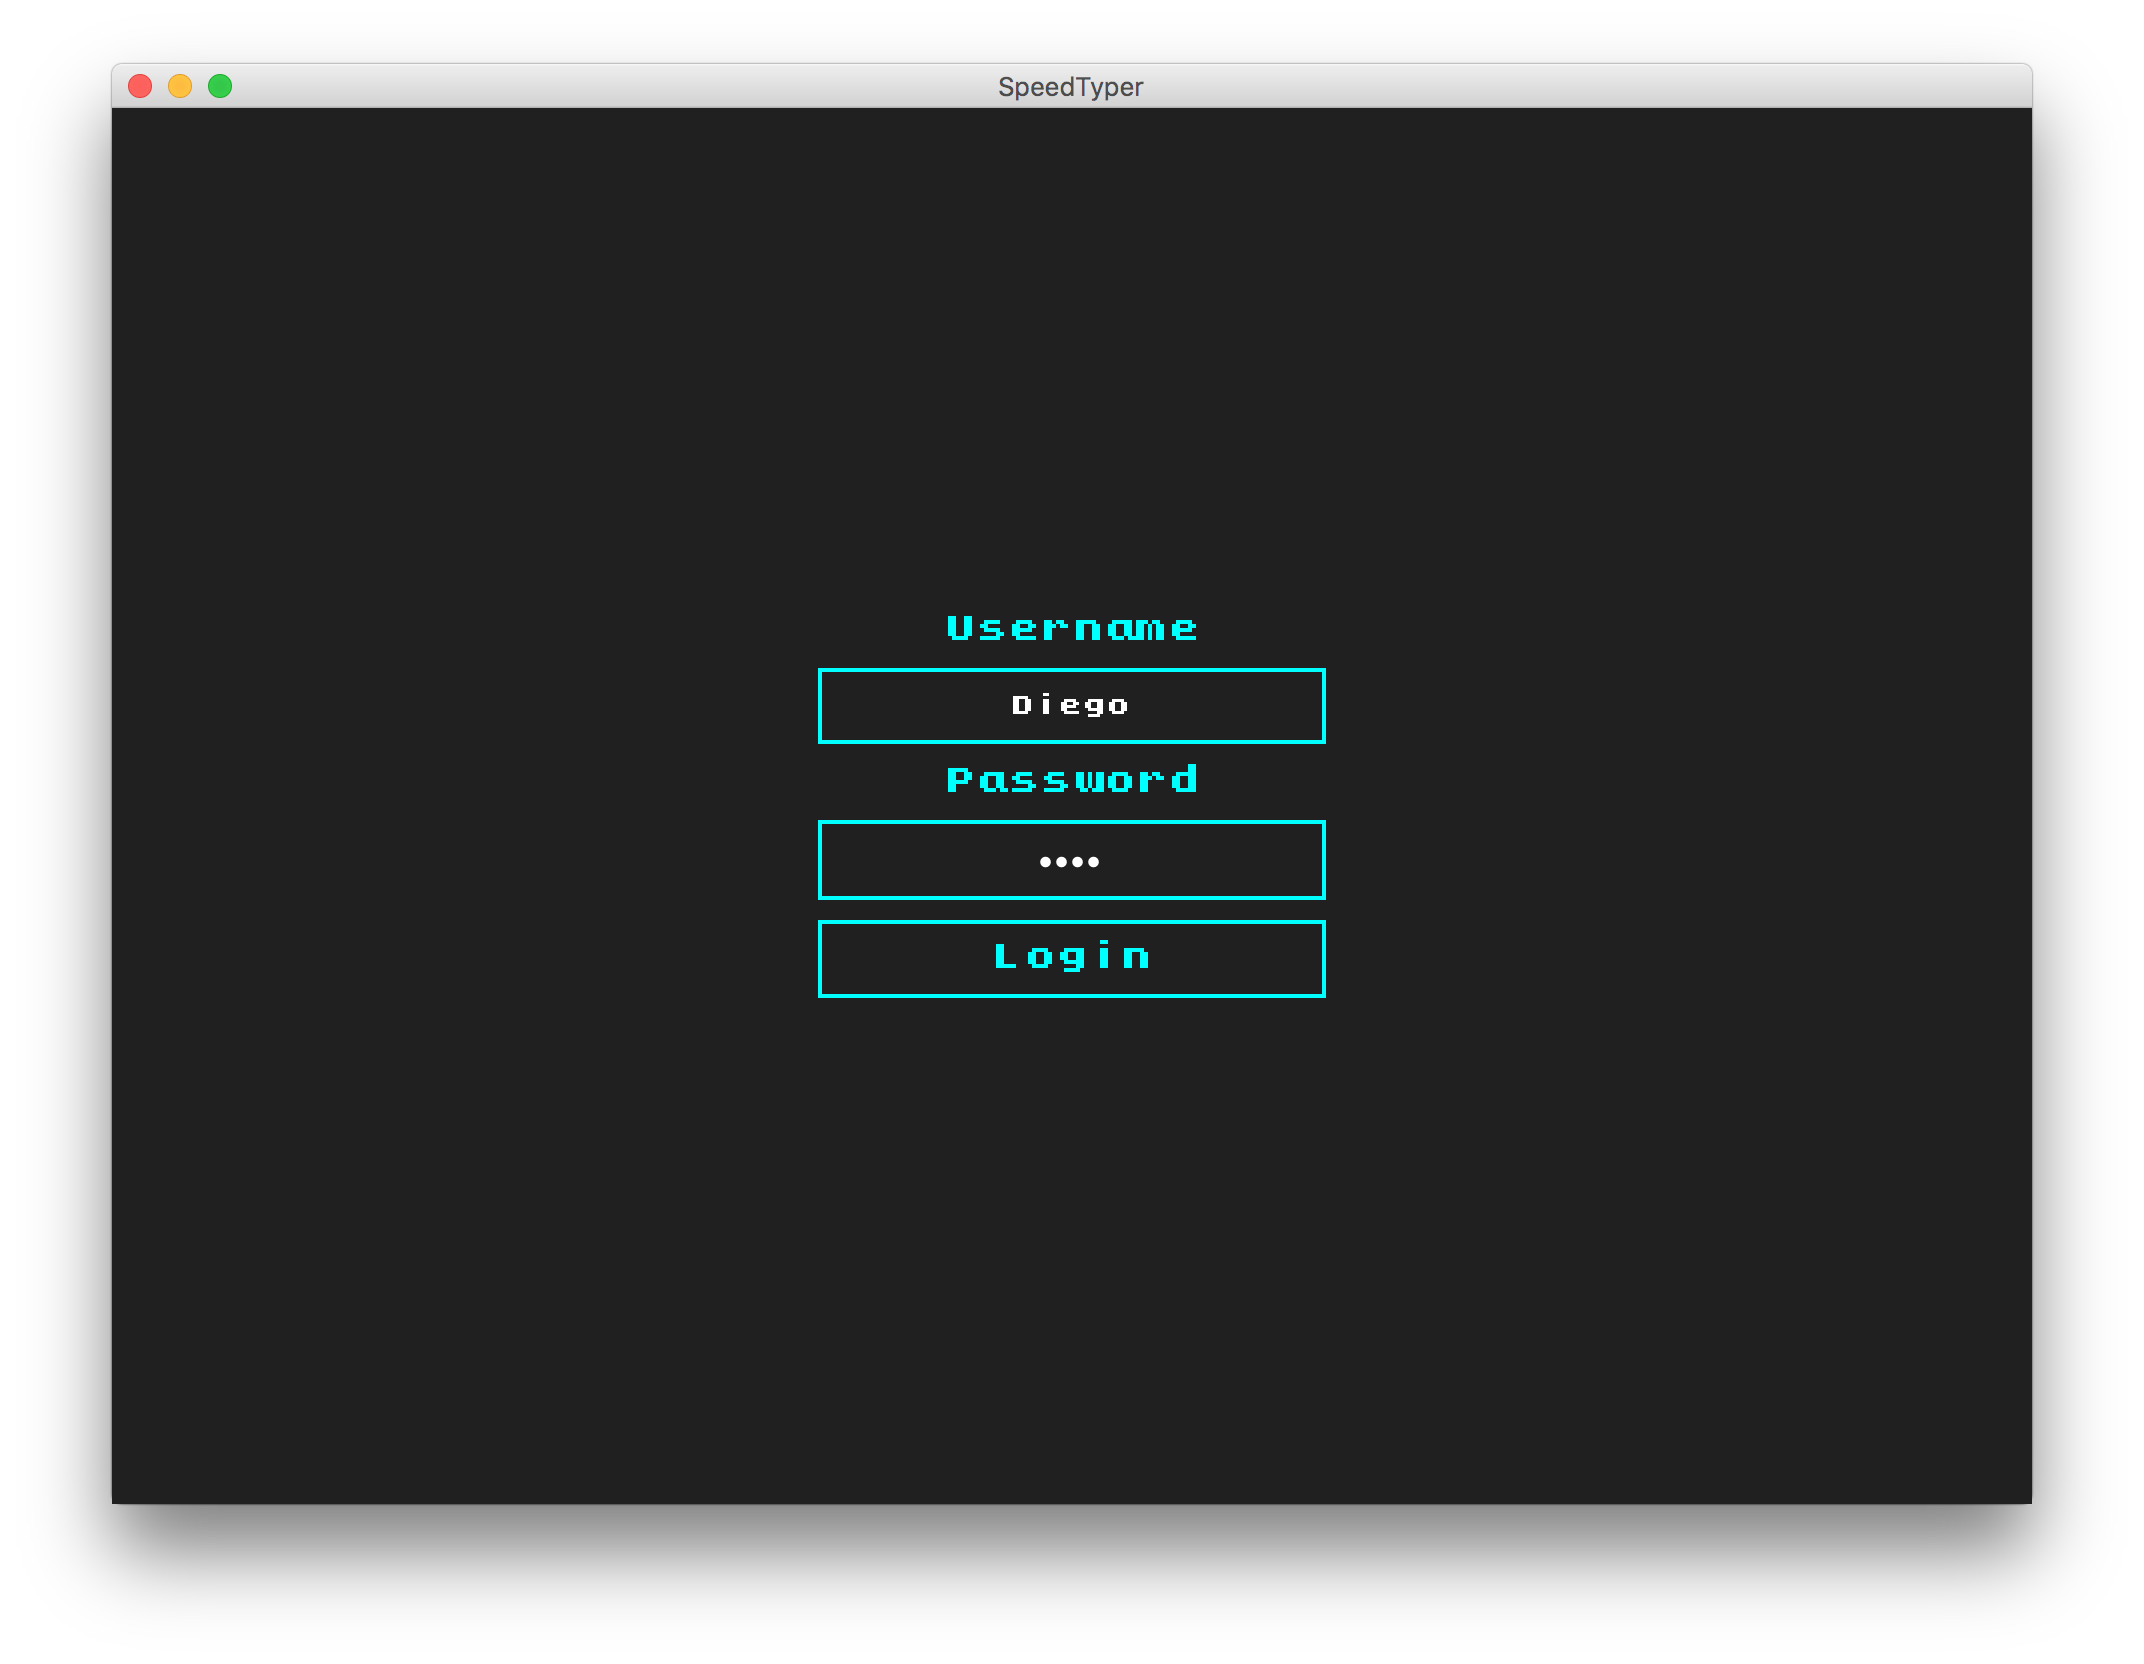
\includegraphics[width=0.7\columnwidth]{../screenshots/login.png}%
				\caption{Screenshot of the login screen}%
				\label{fig:login}%
			\end{figure}
			
			The second one as shown in figure \ref{fig:game} has two fields again: the first one is where the user will type the words and the second one will show to the user the incorrect words he has typed. The user will only be able to type only after pressing the start button (the timer will start at the same time). During the typing, a word can become red: this means that the user has typed something that isn't the prefix of any word and, so, that a mistake has been made. 
			
			\begin{figure}[H]
				\centering
				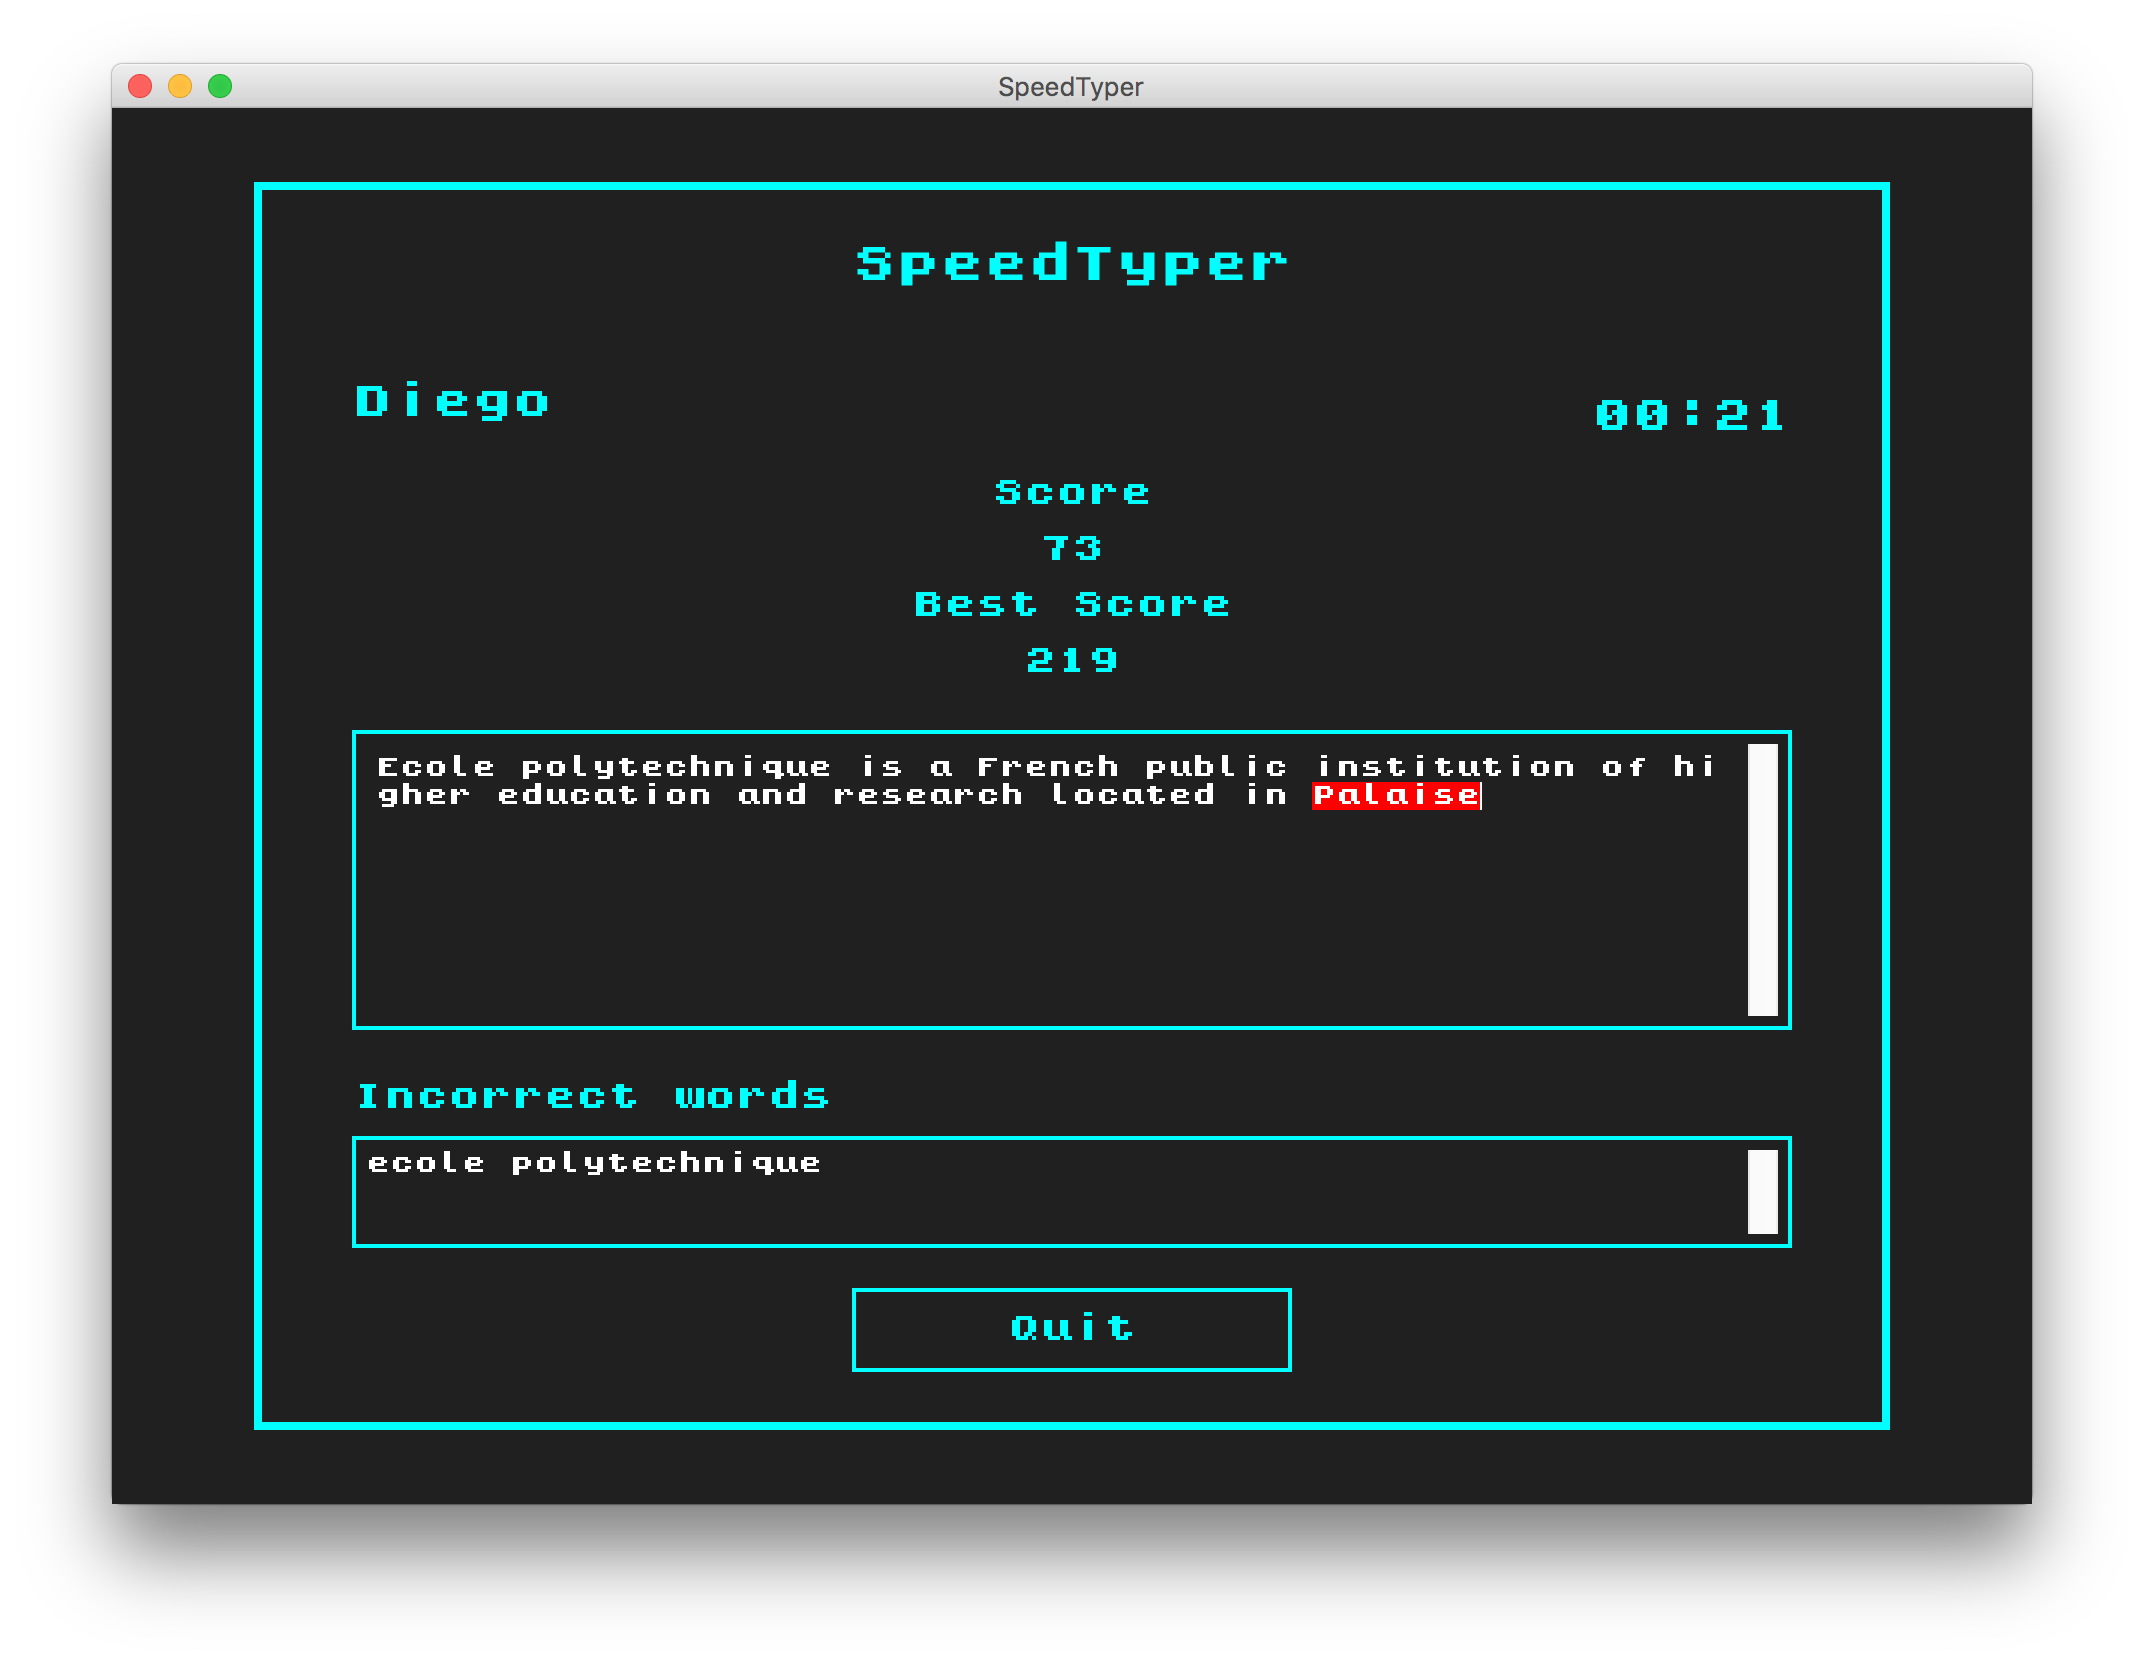
\includegraphics[width=0.7\columnwidth]{../screenshots/typing.png}%
				\caption{Screenshot of the game itself}%
				\label{fig:game}%
			\end{figure}
		
		\subsection{The User Authentication System}
		
			Due to safety reasons, the user authentication system is based in a cryptographic approach. Instead of saving the user password, the software only saves for each user a random sequence of bits (\emph{salt}) and a hash value (given by an one-way function) of the password concatenated with the \emph{salt}. Whenever one registered user tries to login again, it must present a password that when concatenated with the saved \emph{salt} has a hash value equals to the saved hash. The use of a hash function allows higher security than saving the password in plain text: since the knowledge of the hash says nothing about the real password, even if the database is stolen, the users informations would still be safe. The use of the salt increases security too but because it can prevent a precomputed dictionary attack.
		
			The chosen hash function was the SHA-1 and the used implementation is one from the Java libraries (considered to be much safer than writing a new one). Even thought, SHA-1 is not considered the safest hash algorithm anymore, it's safe enough for this project, which, for the moment, won't be the target of many crypto-attacks.
		
		\subsection{The Dictionary Structure}
		
			The dictionary data structure is based in a prefix tree and a very large subset of the English dictionary usually found in most of linux distributions (at \texttt{/usr/share/dict/words}). For simplifying the implementation, all words with non-ASCII characters (such as letters with diacritics) were replaced by the closest ASCII equivalent. 
			
			At the beginning of each execution of the game, the dictionary is loaded into the prefix tree by a class named \texttt{Explorer}. This class, as the name suggests, is the responsible for exploring the prefix tree looking for a typed word by the user. For doing so, this class has: a pointer to the current node of the exploration; a stack of pointers of the previous nodes of the exploration; a counter of wrong letters; and a boolean that indicates if there's a word in the tree with the prefix typed.
			
			With all this attributes, the class is able to: explore the word while the user is still typing it and tell, in real time, if the user has typed a prefix that doesn't correspond to any word in the dictionary. 
			
		\subsection{Future Improvements}
			
			During the execution of this project, many ideas that were conceived couldn't be implemented due to time constraints. The most remarkable ones are:
			
			\begin{itemize}
				\item Creating of a guided typing mode where the user receives a phrase that must be typed;
				\item Querying an online dictionary for getting the words;
				\item Creating a devoted screen for the creation of new users;
				\item Improving the interaction of the user with the game;
				\item Implementing an automatic music for the game.
			\end{itemize}
			
	\section{Conclusion}
	
		Despite having many features that could be improved, this project can be seen as a pretty good implementation of a speed typing game. Many desired features do not require special knowledge and could be done by the developers in a matter of time. So, a future development of this game could lead to a real game that could be deployed for many users.
	
\end{document}